\documentclass[tikz,border=5pt]{standalone}
\usepackage{amsmath,amssymb}
\begin{document}
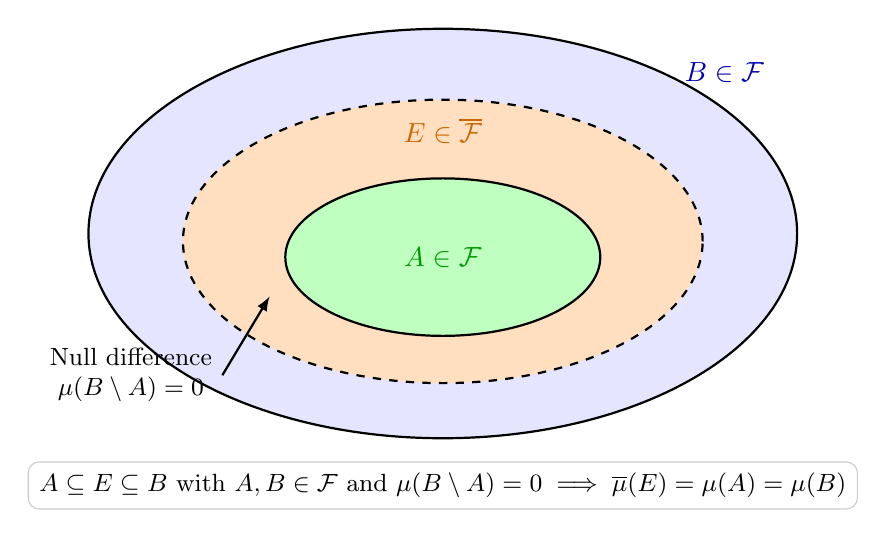
\begin{tikzpicture}[>=latex, font=\small]
  % Outer set B in F
  \draw[thick, fill=blue!10] (0, 0) ellipse (4.5cm and 2.6cm);
  \node[anchor=north east, font=\bfseries, blue!70!black] at (4.2, 2.3) {$B \in \mathcal{F}$};

  % Middle set E in F_bar
  \draw[thick, dashed, fill=orange!25] (0, -0.1) ellipse (3.3cm and 1.8cm);
  \node[font=\bfseries, orange!80!black] at (0, 1.3) {$E \in \overline{\mathcal{F}}$};

  % Inner set A in F
  \draw[thick, fill=green!25] (0, -0.3) ellipse (2.0cm and 1.0cm);
  \node[font=\bfseries, green!60!black] at (0, -0.3) {$A \in \mathcal{F}$};

  % Annotations
  \draw[->, thick] (-2.8, -1.8) node[left, align=center] {Null difference\\$\mu(B \setminus A) = 0$} -- (-2.2, -0.8);
  \node[align=center, fill=white, draw=gray!40, rounded corners, inner sep=4pt] at (0, -3.2)
    {$A \subseteq E \subseteq B$ with $A, B \in \mathcal{F}$ and $\mu(B \setminus A) = 0 \implies \overline{\mu}(E) = \mu(A) = \mu(B)$};
\end{tikzpicture}
\end{document}
